\documentclass[12pt]{article}

\pagestyle{empty}
\setcounter{secnumdepth}{2}

\topmargin=0cm
\oddsidemargin=0cm
\textheight=22.0cm
\textwidth=16cm
\parindent=0cm
\parskip=0.15cm
\topskip=0truecm
\raggedbottom
\abovedisplayskip=3mm
\belowdisplayskip=3mm
\abovedisplayshortskip=0mm
\belowdisplayshortskip=2mm
\normalbaselineskip=12pt
\normalbaselines

\usepackage{graphicx}
\usepackage{float}
\usepackage{titlesec}
\usepackage{pdflscape}

\setcounter{secnumdepth}{3}
\pagenumbering{arabic}
\pagestyle{plain}

\begin{document}

\vspace*{0.5in}
\centerline{\bf\Large Test Document}

\vspace*{0.5in}
\centerline{\bf\Large Team PB-PI}

\vspace*{0.5in}
\centerline{\bf\Large April 8, 2018}

\vspace*{1.5in}
\begin{table}[htbp]
\caption{Team}
\begin{center}
\begin{tabular}{|r | c|}
\hline
Name & ID Number \\
\hline\hline
Alissa Bellerose & 27377320 \\
Sabrina D'Mello & 27739486 \\
Melanie Damilig & 40032420 \\
Tobi Decary-Larocque & 27407645 \\
Zain Farookhi & 26390684 \\
Giulia Gaudio & 27191766 \\
Jason Kalec & 40009464 \\
Damian Kazior & 40016168 \\
Johnny Mak & 40002140 \\
Philip Michael & 40004861 \\
Ramez Nicolas Nahas & 26718108 \\
Steven Tucci & 40006014 \\
Shunyu Wang & 40043915 \\
\hline
\end{tabular}
\end{center}
\end{table}

\clearpage
\tableofcontents
\clearpage

\section{Introduction}

This document contains the overall test plan for the myMoney application. The myMoney application is a tool for young adults and students to keep track of their spending and help with their budgeting. This test plan describes the different tests performed to ensure a working program and explains the reasoning for the tests.\\

The purpose of this document is to provide assurance and show the reliability of the software. The test plan therefore includes:

\begin{itemize}
  \item An overall view of the different tests performed
  \item A description of the tests
  \item References to the use cases and requirements satisfied by testing
\end{itemize}

Testing the program's different functionalities involves different types of tests. Unit, integration and user interface testing were performed for the purpose of this document. This was managed via black-box, white-box and boundary testing.

\section{Test Plan}

For the deposit and withdraw use cases, different unit tests were performed (including boundary tests) to ensure functionality. The different test cases were designed to test each part of each use case. This includes the format of what the user inputs, as well as ensuring that the database is updated or not, according to whether the transaction is legal or not.\\

In regards to our requirements document, the test plan references the deposit and withdrawal use cases specifically. The tests for each of these use cases are integral to the proper functionality of the application and are therefore an important part of the testing sequence. The balance display use case does not have any functional testing to ensure that it works correctly, but any modification to the user's balance should be reflected through the appropriate view. Similarly, the use cases for the ``Show History'' functionality as well as "Export History" do not rely on any user input except for a button click, so testing was only performed to make sure the output files are correct.\\

There were no tests performed to check if the application is portable to all operating systems described in the non-functional requirements, since the application is not being exported as a stand-alone app. It will function within the Eclipse environment for the time being.

\subsection{Use Cases in the myMoney application}

\begin{table}[H]\label{uc}
  \caption{Use Cases (in reference to Requirements Document)}
  \begin{center}
    \begin{tabular}[\textwidth]{|c|c|p{8cm}|}
      \hline
          {\bf Use Case ID} & {\bf Use Case Name} & {\bf Scenario}\\
          \hline
              {\bf UC-1} & Withdraw Money & The user indicates the amount of money they would like to withdraw from the acoount. The system will verify that the account has sufficient funds. Once confirmed, the user request will be processed and the system will subtract the money from the account.

              ALTERNATIVE SCENARIO: The system will deny the request if the user input is not valid or the account does not exist.\\\hline
              
              {\bf UC-2} & Deposit Money & The user indicates the amount they would like to deposit into an account. The system will verify that the input is valid and adds that amount to the specified account.

              A.S.: The user enters invalid input or the account does not exist.\\\hline
              {\bf UC-3} & Display Balance & The user can see the balance of their account. The system will retrieve the amount from the user's specified account.\\\hline
              {\bf UC-4} & Clear Account & The user clears their current account. The system resets to it scleared default state.

              A.S.: The account is already in ``default'' state.\\\hline

              {\bf UC-5} & Show History & The user can view all their deposits and withdrawal transactions that have been entered and processed.\\\hline

              {\bf UC-6} & Sort Table & The user can request to sort their transaction history by certain categories (namely their entered descriptions). The system will sort the information in the way the user requests.\\\hline

                {\bf UC-7} & Export History & The user can request to have the transaction history exported to a separate file. The system will create a .csv file for the user.

                A.S.: The user does not have a transaction history so the request will fail. No file will be produced.\\\hline

    \end{tabular}
  \end{center}
\end{table}

\subsection{System Level Test Cases}

\subsubsection{[TC-1] [Withdraw Money]} \label{tc:1}
%Table 2
\begin{table}[H]
\caption{ TC-1.1 : “Testing the Amount input”}
\begin{center}
\begin{tabular}{|p{5.5	cm}|p{11cm}|}
\hline
\bf Test Case Number & 
TC-1.1 \\
\hline
\bf Description & 
The user enters the amount to withdraw in the “Amount” input text field.\\
\hline
\bf Input & 
\begin{enumerate}
  \item Click Withdraw Money button
  \item Enter the amount as a positive number in Amount input text field environment.
  \item Click Done button
\end{enumerate} \\
\hline
\bf Expected Output & 
\begin{enumerate}
  \item The system records the number from input as “Amount” in a row of transaction history table.
  \item New balance will be updated after deducting the input number from the current Account Balance.
\end{enumerate} \\
\hline
\bf Expected Post-Condition & 
Account balance will be presented as a negative value with two decimal places if it belows 0. Error message is displayed if the input is not valid, 
and Current Balance and database will not be updated.\\
\hline
\bf Execution History & 
[04/14/2018|Shunyu Wang] Executed test successfully.\\
\hline
\bf Trace to Use Case & 
UC-1\\
\hline

\end{tabular}
\end{center}
\end{table}

%Table 3
\begin{table}[H]
\caption{TC-1.2 : “Testing the type of withdraw input”}
\begin{center}
\begin{tabular}{|p{5.5	cm}|p{11cm}|}
\hline
\bf Test Case Number & 
TC-1.2 \\
\hline
\bf Description & 
Takes the type of withdraw defined by the user.\\
\hline
\bf Input & 
\begin{enumerate}
  \item Click Withdraw Money button
  \item Enter any positive number in Amount input text field.
  \item Enter any type of withdraw defined by the user, such as “Bill”, “Check”, or empty string
  \item Click Done button
\end{enumerate} \\
\hline
\bf Expected Output & 
\begin{enumerate}
  \item The system records the number from input as “Amount” and the type of withdraw as “Type of Withdraw” in a row of transaction history table.
  \item New balance will be updated after deducting the input number from the current Account Balance.
\end{enumerate} \\
\hline
\bf Expected Post-Condition & 
The same string will be taken from input as the output for Type of Withdraw in transaction history table. Empty string is allowed.\\
\hline
\bf Execution History & 
[04/14/2018|Shunyu Wang] Executed test successfully.\\
\hline
\bf Trace to Use Case & 
UC-1\\
\hline

\end{tabular}
\end{center}
\end{table}

%Table 4
\begin{table}[H]
\caption{TC-1.3 : “Testing the transaction description input”}
\begin{center}
\begin{tabular}{|p{5.5	cm}|p{11cm}|}
\hline
\bf Test Case Number & 
TC-1.3 \\
\hline
\bf Description & 
Take any user-defined descriptions, such as purposes for transactions and other special notes.\\
\hline
\bf Input & 
\begin{enumerate}
  \item Click Withdraw Money button
  \item Enter any positive number in Amount input text field
  \item Enter any user-defined description in Transaction Description text field, such as “Pay electricity bill of June”, “ Pay off the debt owed to Jack
”, or empty string
  \item Click Done button
\end{enumerate} \\
\hline
\bf Expected Output & 
\begin{enumerate}
  \item The system records the number from input as “Amount” and the user-defined description as “Transaction Description” in a row of transaction history table.
  \item New balance will be updated after deducting the input number from the current Account Balance.
\end{enumerate} \\
\hline
\bf Expected Post-Condition & 
The same string will be taken from input as the output for Transaction Description in transaction history table. Empty string is allowed.\\
\hline
\bf Execution History & 
[04/14/2018|Shunyu Wang] Executed test successfully.\\
\hline
\bf Trace to Use Case & 
UC-1\\
\hline

\end{tabular}
\end{center}
\end{table}


%Table 5
\begin{table}[H]
\caption{TC-1.4 : “Testing the Done UI Button”}
\begin{center}
\begin{tabular}{|p{5.5	cm}|p{11cm}|}
\hline
\bf Test Case Number & 
TC-1.4 \\
\hline
\bf Description & 
When clicked, the UI and the database are updated according to the values entered by the user. In some cases, error messages are displayed.\\
\hline
\bf Input & 
\begin{enumerate}
  \item Click Withdraw Money button
  \item Refer to TC-1.1, TC-1.2, and TC-1.3, input testing data appropriately
  \item Click Done button
\end{enumerate} \\
\hline
\bf Expected Output & 
\begin{enumerate}
  \item The system records the number from input as “Amount”, the type of withdraw as “Type of Withdraw”, and the user-defined description as “Transaction Description” in a row of transaction history table.
  \item New balance will be updated after deducting the input number from the current Account Balance.
\end{enumerate} \\
\hline
\bf Expected Post-Condition & 
Account balance will be presented as a negative value with two decimal places if it falls belows 0. All testing data should be recorded together  in database as a row transaction history, which can be examined by clicking Show History\\
\hline
\bf Execution History & 
[04/14/2018|Shunyu Wang] Executed test successfully.\\
\hline
\bf Trace to Use Case & 
UC-1\\
\hline

\end{tabular}
\end{center}
\end{table}


%Table 6
\begin{table}[H]
\caption{TC-1.5 : “Testing the Cancel UI Button”}
\begin{center}
\begin{tabular}{|p{5.5	cm}|p{11cm}|}
\hline
\bf Test Case Number & 
TC-1.5 \\
\hline
\bf Description & 
When clicked, the transaction is canceled: the Account Balance and database are not updated.\\
\hline
\bf Input & 
\begin{enumerate}
  \item Click Withdraw Money button
  \item Input any testing data into text fields
  \item Click Cancel button
\end{enumerate} \\
\hline
\bf Expected Output & 
\begin{enumerate}
  \item Data are cleared and all input text fields are collapsed.
\end{enumerate} \\
\hline
\bf Expected Post-Condition & 
The system state doesn’t change, meaning Current Balance is not changed and no change in database.\\
\hline
\bf Execution History & 
[04/14/2018|Shunyu Wang] Executed test successfully.\\
\hline
\bf Trace to Use Case & 
UC-1\\
\hline

\end{tabular}
\end{center}
\end{table}

\subsubsection{[TC-2] [Deposit Money]} \label{tc:2}

%Table 7
\begin{table}[H]
\caption{TC-2.1 : “ Testing the amount input”}
\begin{center}
\begin{tabular}{|p{5.5	cm}|p{11cm}|}
\hline
\bf Test Case Number & 
TC-2.1 \\
\hline
\bf Description & 
The user enters the amount to deposit in the “Amount” input text field.\\
\hline
\bf Input & 
\begin{enumerate}
  \item Click Deposit Money button
  \item Enter the amount as a positive number in Amount input text field.
  \item Click Done button
\end{enumerate} \\
\hline
\bf Expected Output & 
\begin{enumerate}
  \item The system records the number from input as “Amount” in a row of transaction history table.
  \item New balance will be updated after adding the input number to the current Account Balance.
\end{enumerate} \\
\hline
\bf Expected Post-Condition & 
Account balance will be presented as a positive value with two decimal places. Error message is displayed if the input is not valid, and Current Balance and database will not be updated.\\
\hline
\bf Execution History & 
[04/14/2018|Shunyu Wang] Executed test successfully.\\
\hline
\bf Trace to Use Case & 
UC-2\\
\hline

\end{tabular}
\end{center}
\end{table}


%Table 8
\begin{table}[H]
\caption{TC-2.2 : “Testing the type of deposit”}
\begin{center}
\begin{tabular}{|p{5.5	cm}|p{11cm}|}
\hline
\bf Test Case Number & 
TC-2.2 \\
\hline
\bf Description & 
Takes the type of deposit defined by the user.\\
\hline
\bf Input & 
\begin{enumerate}
  \item Click Deposit Money button
  \item Enter the amount as a positive number in Amount input text field.
  \item Enter any type of deposit defined by the user, such as “Direct Deposit”, “Cash”, or empty string
  \item Click Done button
\end{enumerate} \\
\hline
\bf Expected Output & 
\begin{enumerate}
  \item The system records the number from input as “Amount” and the type of deposit as “Type of Deposit” in a row of transaction history table.
  \item New balance will be updated after adding the input number to the current Account Balance.
\end{enumerate} \\
\hline
\bf Expected Post-Condition & 
The same string will be taken from input as the output for Type of Deposit in transaction history table. Empty string is allowed.\\
\hline
\bf Execution History & 
[04/14/2018 | Shunyu Wang] Executed test successfully.\\
\hline
\bf Trace to Use Case & 
UC-2\\
\hline

\end{tabular}
\end{center}
\end{table}


%Table 9
\begin{table}[H]
\caption{TC-2.3 : “Testing the transaction description input”}
\begin{center}
\begin{tabular}{|p{5.5	cm}|p{11cm}|}
\hline
\bf Test Case Number & 
TC-2.3 \\
\hline
\bf Description & 
Take any user-defined descriptions, such as purposes for transactions and other special notes.\\
\hline
\bf Input & 
\begin{enumerate}
  \item Click Deposit Money button
  \item Enter the amount as a positive number in Amount input text field.
  \item Enter any user-defined description in Transaction Description text field, such as “Bi-weekly pay”, “Receive the bonus for working overtime”, or empty string.
  \item Click Done button
\end{enumerate} \\
\hline
\bf Expected Output & 
\begin{enumerate}
  \item The system records the number from input as “Amount” and the user-defined description as “Transaction Description” in a row of transaction history table
  \item New balance will be updated after adding the input number to the current Account Balance
\end{enumerate} \\
\hline
\bf Expected Post-Condition & 
The same string will be taken from input as the output for Transaction Description in transaction history table. Empty string is allowed.\\
\hline
\bf Execution History & 
[04/14/2018 | Shunyu Wang] Executed test successfully.\\
\hline
\bf Trace to Use Case & 
UC-2\\
\hline

\end{tabular}
\end{center}
\end{table}


%Table 10
\begin{table}[H]
\caption{TC-2.4 : “Testing the Done UI Button”}
\begin{center}
\begin{tabular}{|p{5.5	cm}|p{11cm}|}
\hline
\bf Test Case Number & 
TC-2.4 \\
\hline
\bf Description & 
When clicked, the UI and the database are updated according to the values entered by the user. In some cases, error messages are displayed.\\
\hline
\bf Input & 
\begin{enumerate}
  \item Click Deposit Money button
  \item Refer to TC-2.1, TC-2.2, and TC-2.3, input testing data appropriately. string.
  \item Click Done button
\end{enumerate} \\
\hline
\bf Expected Output & 
\begin{enumerate}
  \item The system records the number from input as “Amount”, the type of deposit as “Type of Deposit”, and the user-defined description as “Transaction Description” in a row of transaction history table.
  \item New balance will be updated after adding the input number to current Account Balance.
\end{enumerate} \\
\hline
\bf Expected Post-Condition & 
Account balance will be presented as a negative value with two decimal places if it falls belows 0. All testing data should be recorded together  in database as a row transaction history, which can be examined by clicking Show History\\
\hline
\bf Execution History & 
[04/14/2018 | Shunyu Wang] Executed test successfully.\\
\hline
\bf Trace to Use Case & 
UC-2\\
\hline

\end{tabular}
\end{center}
\end{table}


%Table 11
\begin{table}[H]
\caption{TC-2.5 : “Testing the Cancel UI Button”}
\begin{center}
\begin{tabular}{|p{5.5	cm}|p{11cm}|}
\hline
\bf Test Case Number & 
TC-2.5 \\
\hline
\bf Description & 
When clicked, the transaction is canceled: the UI and database are not updated.\\
\hline
\bf Input & 
\begin{enumerate}
  \item Click Deposit Money button
  \item Input any testing data into text fields
  \item Click Cancel button
\end{enumerate} \\
\hline
\bf Expected Output & 
\begin{enumerate}
  \item All data are cleared and all input text fields are collapsed.
\end{enumerate} \\
\hline
\bf Expected Post-Condition & 
The system state doesn’t change, meaning Current Balance is not changed and no change in database\\
\hline
\bf Execution History & 
[04/14/2018 | Shunyu Wang] Executed test successfully.\\
\hline
\bf Trace to Use Case & 
UC-2\\
\hline

\end{tabular}
\end{center}
\end{table}

\subsubsection{[TC-3] [Display Balance]} \label{tc:3}

%Table 12
\begin{table}[H]
\caption{TC-3.1 : “Testing the Display Balance”}
\begin{center}
\begin{tabular}{|p{5.5	cm}|p{11cm}|}
\hline
\bf Test Case Number & TC-3.1\\
\hline
\bf Description & This test is used to show the balance is properly displaying the correct amount from the user's account.\\
\hline
\bf Input &
\begin{enumerate}
\item The user opens the application.
\item The user sees the balance displayed in the lower center area of the default application window.
\end{enumerate}
\\
\hline
\bf Expected Output &
\begin{enumerate}
\item The system will query the database.
\item The balance is displayed on the screen.
\end{enumerate}
\\
\hline
\bf Expected Post-Condition & The application will display the balance in green if the amount in the account is positive, and in red if the account is negative.\\
\hline
\bf Execution History & [04/14/18 | Sabrina D'Mello] Executed test successfully.\\
\hline
\bf Trace to Use Case & UC-3\\
\hline

\end{tabular}
\end{center}
\end{table}

\subsubsection{[TC-4] [Clear Account]} \label{tc:4}

%Table 13
\begin{table}[H]
\caption{TC-4.1 : “Testing Clear Account”}
\begin{center}
\begin{tabular}{|p{5.5	cm}|p{11cm}|}
\hline
\bf Test Case Number & TC-4.1\\
\hline
\bf Description & Ensure that all transaction records for the account are deleted after user clicks on ``Clear Account''.\\
\hline
\bf Input &
\begin{enumerate}
\item The user makes at least one deposit or withdrawal transaction from the account (see UC-1 and UC-2).
\item The user clicks on ``Clear Account''.
\end{enumerate}
\\
\hline
\bf Expected Output &
\begin{enumerate}
\item The account balance is reset to 0.00\$.
\item All transactions are removed from the account database.
\end{enumerate}
\\
\hline
\bf Expected Post-Condition & The entire account is reset to a default state. If the system was already in a default state, no observable changes will take place.\\
\hline
\bf Execution History & [04/14/2018 | Shunyu Wang] Executed test successfully.\\
\hline
\bf Trace to Use Case & UC-1, UC-2, UC-4.\\\hline
\end{tabular}
\end{center}
\end{table}

\subsubsection{[TC-5] [Show History]} \label{tc:5}

%Table 14
\begin{table}[H]
\caption{TC-5.1 : “Testing Show History”}
\begin{center}
\begin{tabular}{|p{5.5	cm}|p{11cm}|}
\hline
\bf Test Case Number & TC-5.1\\
\hline
\bf Description & This test case ensures the functionality of Show History, which shows a history of all deposit and withdrawal transactions. Additionally, information such as the type of transaction, the reason and dates should all be present.\\
\hline
\bf Input &
\begin{enumerate}
\item User clicks ``Show History'' button.
\end{enumerate}
\\
\hline
\bf Expected Output &
\begin{enumerate}
\item New GUI window opens.
\item All information for a given transaction is presented on a line.
\end{enumerate}
\\
\hline
\bf Expected Post-Condition & Separate window opens.\\\hline
\bf Execution History & [04/15/2018 | Philip Michael] Executed test successfully.\\\hline
\bf Trace to Use Case & UC-5 \\

\hline
\end{tabular}
\end{center}
\end{table}

\subsubsection{[TC-6] [Sort Table]} \label{tc:6}

%Table 15
\begin{table}[H]
\caption{TC-6.1 : “Testing Sort by Date”}
\begin{center}
\begin{tabular}{|p{5.5	cm}|p{11cm}|}
  \hline
  \bf Test Case Number & TC-6.1\\\hline
  \bf Description & This test case ensures that sorting by date functions properly in the Transaction History GUI window that is accessed through the ``Show History'' button on the landing GUI.\\\hline
  \bf Input &
  \begin{enumerate}
  \item User opens Transaction History
  \item User clicks on ``Date'' column header
  \end{enumerate}
  \\\hline
  \bf Expected Output &
  \begin{enumerate}
  \item Transactions are sorted by descending date, if arrow is pointing up.
  \item Transactions are sorted by date ascending, if arrow is pointed down.
  \item If no arrow is shown, no sorting is performed.
  \end{enumerate}
  \\\hline
  \bf Expected Post-Condition & The data is sorted according to the state it is in.\\\hline
  \bf Execution History & [04/15/2018 | Philip Michael] Executed test succesfully.\\\hline
  \bf Trace to Use Case & UC-5, UC-6\\

  \hline
\end{tabular}
\end{center}
\end{table}

%Table 16
\begin{table}[H]
\caption{TC-6.2 : “Testing Sort by Transaction Type”}
\begin{center}
\begin{tabular}{|p{5.5	cm}|p{11cm}|}
  \hline
  \bf Test Case Number & TC-6.2\\\hline
  \bf Description & This test case ensures that sorting by transaction type functions properly in the Transaction History GUI window that is accessed through the ``Show History'' button on the landing GUI.\\\hline
  \bf Input &
  \begin{enumerate}
  \item User opens Transaction History
  \item User clicks on ``Transation Type'' column header
  \end{enumerate}
  \\\hline
  \bf Expected Output &
  \begin{enumerate}
  \item Transactions are sorted by deposit first, if arrow is pointing up.
  \item Transactions are sorted by withdrawal first, if arrow is pointed down.
  \item If no arrow is shown, no sorting is performed.
  \end{enumerate}
  \\\hline
  \bf Expected Post-Condition & The data is sorted according to the state it is in.\\\hline
  \bf Execution History & [04/15/2018 | Philip Michael] Executed test succesfully.\\\hline
  \bf Trace to Use Case & UC-5, UC-6\\

  \hline
\end{tabular}
\end{center}
\end{table}

%Table 17
\begin{table}[H]
\caption{TC-6.3 : “Testing Sort by Description”}
\begin{center}
\begin{tabular}{|p{5.5	cm}|p{11cm}|}
  \hline
  \bf Test Case Number & TC-6.3\\\hline
  \bf Description & This test case ensures that sorting by description functions properly in the Transaction History GUI window that is accessed through the ``Show History'' button on the landing GUI.\\\hline
  \bf Input &
  \begin{enumerate}
  \item User opens Transaction History
  \item User clicks on ``Description'' column header
  \end{enumerate}
  \\\hline
  \bf Expected Output &
  \begin{enumerate}
  \item Transactions are sorted alphabetically, if arrow is pointing up.
  \item Transactions are sorted in reverse alphabetical order, if arrow is pointed down.
  \item If no arrow is shown, no sorting is performed.
  \end{enumerate}
  \\\hline
  \bf Expected Post-Condition & The data is sorted according to the state it is in.\\\hline
  \bf Execution History & [04/15/2018 | Philip Michael] Executed test succesfully.\\\hline
  \bf Trace to Use Case & UC-5, UC-6\\

  \hline
\end{tabular}
\end{center}
\end{table}

%Table 18
\begin{table}[H]
\caption{TC-6.4 : “Testing Sort by Amount”}
\begin{center}
\begin{tabular}{|p{5.5	cm}|p{11cm}|}
  \hline
  \bf Test Case Number & TC-6.4\\\hline
  \bf Description & This test case ensures that sorting by amount functions properly in the Transaction History GUI window that is accessed through the ``Show History'' button on the landing GUI.\\\hline
  \bf Input &
  \begin{enumerate}
  \item User opens Transaction History
  \item User clicks on ``Amount'' column header
  \end{enumerate}
  \\\hline
  \bf Expected Output &
  \begin{enumerate}
  \item Transactions are sorted by ascending amount, if arrow is pointing up.
  \item Transactions are sorted by descending amount, if arrow is pointed down.
  \item If no arrow is shown, no sorting is performed.
  \end{enumerate}
  \\\hline
  \bf Expected Post-Condition & The data is sorted according to the state it is in.\\\hline
  \bf Execution History & [04/15/2018 | Philip Michael] Executed test succesfully.\\\hline
  \bf Trace to Use Case & UC-5, UC-6\\

  \hline
\end{tabular}
\end{center}
\end{table}

%Table 19
\begin{table}[H]
\caption{TC-6.5 : “Testing Sort by Withdrawal Type”}
\begin{center}
\begin{tabular}{|p{5.5	cm}|p{11cm}|}
  \hline
  \bf Test Case Number & TC-6.5\\\hline
  \bf Description & This test case ensures that sorting by withdrawal type functions properly in the Transaction History GUI window that is accessed through the ``Show History'' button on the landing GUI.\\\hline
  \bf Input &
  \begin{enumerate}
  \item User opens Transaction History
  \item User clicks on ``Type of Withdrawal'' column header
  \end{enumerate}
  \\\hline
  \bf Expected Output &
  \begin{enumerate}
  \item Transactions are sorted alphabetically, if arrow is pointing up.
  \item Transactions are sorted in reverse alphabetical order, if arrow is pointed down.
  \item If no arrow is shown, no sorting is performed.
  \end{enumerate}
  \\\hline
  \bf Expected Post-Condition & The data is sorted according to the state it is in.\\\hline
  \bf Execution History & [04/15/2018 | Philip Michael] Executed test succesfully.\\\hline
  \bf Trace to Use Case & UC-5, UC-6\\

  \hline
\end{tabular}
\end{center}
\end{table}

%Table 20
\begin{table}[H]
\caption{TC-6.6 : “Testing Sort by Deposit Type”}
\begin{center}
\begin{tabular}{|p{5.5	cm}|p{11cm}|}
  \hline
  \bf Test Case Number & TC-6.6\\\hline
  \bf Description & This test case ensures that sorting by deposit type functions properly in the Transaction History GUI window that is accessed through the ``Show History'' button on the landing GUI.\\\hline
  \bf Input &
  \begin{enumerate}
  \item User opens Transaction History
  \item User clicks on ``Type of Deposit'' column header
  \end{enumerate}
  \\\hline
  \bf Expected Output &
  \begin{enumerate}
  \item Transactions are sorted alphabetically, if arrow is pointing up.
  \item Transactions are sorted in reverse alphabetical order, if arrow is pointed down.
  \item If no arrow is shown, no sorting is performed.
  \end{enumerate}
  \\\hline
  \bf Expected Post-Condition & The data is sorted according to the state it is in.\\\hline
  \bf Execution History & [04/15/2018 | Philip Michael] Executed test succesfully.\\\hline
  \bf Trace to Use Case & UC-5, UC-6\\

  \hline
\end{tabular}
\end{center}
\end{table}

\subsubsection{[TC-7] [Export History]} \label{tc:7}

%Table 20
\begin{table}[H]
\caption{TC-7.1 : “Testing Export History”}
\begin{center}
\begin{tabular}{|p{5.5	cm}|p{11cm}|}
  \hline
  \bf Test Case Number & TC-7.1\\\hline
  \bf Description & Verify that the user can download a .csv file of their transaction history.\\\hline
  \bf Input &
  \begin{enumerate}
  \item User performs at least one deposit or withdrawal transaction.
  \item User clicks on ``Export History'' button in the Advanced Options
  \end{enumerate}
  \\\hline
  \bf Expected Output &
  \begin{enumerate}
  \item A .csv file is created and saved in a default location.
  \end{enumerate}
  \\\hline
  \bf Expected Post-Condition & The data from the file is sorted according to the state it is in.\\\hline
  \bf Execution History & [04/15/2018 | Sabrina D'Mello] Executed test succesfully.\\\hline
  \bf Trace to Use Case & UC-6, UC-7\\

  \hline
\end{tabular}
\end{center}
\end{table}

\section{Unit Test Cases}

\subsection{Display Balance Unit Testing} \label{ut:1}

%Table 21
\begin{table}[H]
\caption{“initialBalanceTest()”}
\begin{center}
\begin{tabular}{|p{5.5cm}|p{11cm}|}
  \hline
  \bf Test Case Number & UT-1\\\hline
  \bf Description & 
  This unit test case is used to ensure that when the myMoney application is initially opened that it will display the current historical balance on the account.\\\hline
  \bf Input &
  \begin{enumerate}
  \item .......
  \end{enumerate}
  \\\hline
  \bf Expected Output &
  \begin{enumerate}
  \item Test was executed successfully
  \end{enumerate}
  \\\hline
  \bf Expected Post-Condition & 
  ..............
  \\\hline   
  \bf Execution History & 
  \begin{enumerate}
  \item (04/15/2018) Sabrina D’Mello: Executed test successfully.
  \item (04/6/201) Damian Kazior Executed test successfully.
  \end{enumerate}
  \\\hline
\end{tabular}
\end{center}
\end{table}

%Table 22
\begin{table}[H]
\caption{“updateBalanceTest()”}
\begin{center}
\begin{tabular}{|p{5.5cm}|p{11cm}|}
  \hline
  \bf Test Case Number & UT-2\\\hline
  \bf Description & 
  This unit test case is used to ensure that the system updates the balance positively or negatively, depending on the transaction type.\\\hline
  \bf Input &
  \begin{enumerate}
  \item .......
  \end{enumerate}
  \\\hline
  \bf Expected Output &
  \begin{enumerate}
  \item Test was executed successfully
  \end{enumerate}
  \\\hline
  \bf Expected Post-Condition & 
  ..............
  \\\hline   
  \bf Execution History & 
  \begin{enumerate}
  \item (04/15/2018) Sabrina D’Mello: Executed test successfully.
  \item (04/6/201) Damian Kazior Executed test successfully.
  \end{enumerate}
  \\\hline
\end{tabular}
\end{center}
\end{table}

%Table 23
\begin{table}[H]
\caption{“updateModelTest()”}
\begin{center}
\begin{tabular}{|p{5.5cm}|p{11cm}|}
  \hline
  \bf Test Case Number & UT-3\\\hline
  \bf Description & 
  This unit test case was created to ensure that the model  updates once a change has been made to the view.\\\hline
  \bf Input &
  \begin{enumerate}
  \item .......
  \end{enumerate}
  \\\hline
  \bf Expected Output &
  \begin{enumerate}
  \item Test was executed successfully
  \end{enumerate}
  \\\hline
  \bf Expected Post-Condition & 
  ..............
  \\\hline   
  \bf Execution History & 
  \begin{enumerate}
  \item (04/15/2018) Sabrina D’Mello: Executed test successfully.
  \item (04/6/201) Damian Kazior Executed test successfully.
  \end{enumerate}
  \\\hline
\end{tabular}
\end{center}
\end{table}


\subsection{Data Unit Testing} \label{ut:2}

%Table 24
\begin{table}[H]
\caption{“CreateDummyDeposit()”}
\begin{center}
\begin{tabular}{|p{5.5cm}|p{11cm}|}
  \hline
  \bf Test Case Number & UT-4\\\hline
  \bf Description & 
This unit test case was to ensure that the database fields in the deposit money model is being set and the amount is being added it correctly.\\\hline
  \bf Input &
  \begin{enumerate}
  \item .......
  \end{enumerate}
  \\\hline
  \bf Expected Output &
  \begin{enumerate}
  \item Test was executed successfully
  \end{enumerate}
  \\\hline
  \bf Expected Post-Condition & 
  ..............
  \\\hline   
  \bf Execution History & 
  \begin{enumerate}
  \item (04/15/2018) Sabrina D’Mello: Executed test successfully.
  \item (04/6/201) Damian Kazior Executed test successfully.
  \end{enumerate}
  \\\hline
\end{tabular}
\end{center}
\end{table}

%Table 25
\begin{table}[H]
\caption{“CreateDummyWithdrawal()”}
\begin{center}
\begin{tabular}{|p{5.5cm}|p{11cm}|}
  \hline
  \bf Test Case Number & UT-5	\\\hline
  \bf Description & 
This unit test case was to ensure that the database fields in the withdraw money model is being set and the amount is being deducted correctly.\\\hline
  \bf Input &
  \begin{enumerate}
  \item .......
  \end{enumerate}
  \\\hline
  \bf Expected Output &
  \begin{enumerate}
  \item Test was executed successfully
  \end{enumerate}
  \\\hline
  \bf Expected Post-Condition & 
  ..............
  \\\hline   
  \bf Execution History & 
  \begin{enumerate}
  \item (04/15/2018) Sabrina D’Mello: Executed test successfully.
  \item (04/6/201) Damian Kazior Executed test successfully.
  \end{enumerate}
  \\\hline
\end{tabular}
\end{center}
\end{table}

\section{Test Results}

In this section we will be outlining the test results for both of our main test cases while providing in depth information regarding regular, special, and boundary cases. 

\subsection{Deposit Money Test}

1. Expected Output (when ``Done'' button is clicked, and tests are implemented in order\\

Regular Cases
\begin{itemize}
  \item Value 100: Works as expected.\\
Account: 100.00 Current Balance: 100.00
  \item Value 200.78: Works as expected.\\
Account: 300.78 Current Balance: 300.78
\end{itemize}

Special Cases
\begin{itemize}
  \item Value -50: Does not work as expected. Subtracts 50 from the account and from the ``Current Balance'' field.\\
No error message is displayed.
  \item Value ``Hello'': Works as expected. An error message appears.\\
Error: Value entered must be a positive number.
  \item Value: 3.2222: Works as expected.\\
Account: 304.0022 Current Balance: 304.00
  \item Value -30.55: Subtracts 30.55 from the account and from the ``Current Balance'' field.\\
No error message is displayed.
\end{itemize}

2. Type of Deposit'' input text field\\

Boundary Cases
\begin{itemize}
  \item Pass nothing (leave the field empty). Works as expected. The deposit concludes with default reason.
\end{itemize}

Regular Cases
\begin{itemize}
  \item Pass a string  ``Cash Entry''. Works as expected and provides deposit reason.
  \item Pass a string containing a number  ``Money Transfer \#3''. Works as expected and provides deposit reason.
\end{itemize}

3. ``(optional) Transaction Description" input text field \\

Boundary Cases
\begin{itemize}
  \item Pass nothing (leave the field empty). Works as expected with no description.
\end{itemize}

Regular Cases
\begin{itemize}
  \item Pass a string ``Money found in couch''. Works as expected and provides description.
  \item Pass a string containing a number ``Sold Xbox 360''. Works as expected and provides description.
\end{itemize}

4. ``Done" button\\

All tests above satisfy this case as they require the use of the Done button. Please refer to sections 1 and 2.\\
	
5. ``Cancel" button\\

Regular Cases
\begin{itemize}
  \item Transaction is not recorded. That is:
  \begin{itemize}
    \item Account (database) does not contain a record corresponding to the input. Works as expected.
    \item ``Current Balance field'' is unchanged. Works as expected.
  \end{itemize}
\end{itemize}

\subsection{Withdraw Money Test}

1. Expected Output (when ``Done'' button is clicked, and tests are implemented in order)\\

Boundary Cases:
\begin{itemize}
  \item Passing a 0 or a 0.00: Works as expected, no actual change is done to the balance.
\end{itemize}

Regular Cases:
\begin{itemize}
  \item Value of 100: Works as expected, withdrawal is performed.
  \item Value of 200.78: Works as expected. Withdrawal is performed.
\end{itemize}

Special Cases:
\begin{itemize}
  \item Value of -50: Does not work as expected.  It adds 50 to the account and to the ``Current Balance'' field. No error message is shown.
  \item Value ``Hello'': Works as expected. An error message is shown.
  \item Value 3.2222: Works as expected by being rounded to the nearest hundredth when performing the withdrawal. 
\end{itemize}

2. Expected Output (when ``Show History'' is clicked).\\

Boundary Cases:
\begin{itemize}
  \item ``'' is under the ``TYPE OF WITHDRAW'': Works as expected. It is left blank.
\end{itemize}

Regular Cases:
\begin{itemize}
  \item ``bill'' is under the ``TYPE OF WITHDRAW'': Works as expected. Bill is shown as the type of the withdrawal.
  \item ``check'' is under the ``TYPE OF WITHDRAW'': Works as expected. Check is shown as the type of the withdrawal.
\end{itemize}

3. (optional) ``Transaction Description'' input text field\\

Boundary Cases:
\begin{itemize}
  \item ``'' is under the ``DESCRIPTION'': Works as expected. It is left blank.
\end{itemize}

Regular Cases:
\begin{itemize}
  \item  ``Pay electricity bill of June'' is under the ``DESCRIPTION'': Works as expected. Shows this as the description for the withdrawal.
  \item  ``Pay off the debt owed to Jack'' is under the ``DESCRIPTION'': Works as expected. Shows this as the description for the withdrawal.
\end{itemize}

4. ``Done'' button\\

Expected output is relative to the outlined uses in the above cases. They all require the use of the ``Done'' button, therefore this button is tested through those same tests.\\
	
5. ``Cancel'' button\\

Regular Cases:
\begin{itemize}
  \item Transaction is not recorded. That is:
  \begin{itemize}
    \item Account (database) does not contain a record corresponding to input data: Works as expected.
    \item ``Current Balance'' field is unchanged: Works as expected. No changes occur.
  \end{itemize}
\end{itemize}

\section{References}
We obtained a test document sample that we used as a reference: Montrealopoly, Master Test Plan, from: https://users.encs.concordia.ca/~paquet/wiki/images/3/35/Phase3final.pdf

\appendix

\section{Description of Input Files}

%TABLEs REQUIRE FIXING !!!!!

%Table 28
\begin{table}[H]
\caption{Input Files}
\begin{center}
\begin{tabular}{|c|c|p{3cm}|p{2cm}}
\hline
  \bf File Name & \bf File Extension & \bf File Description & \bf Input Description \\\hline
	\bf mymoneyappdb &
		.db &
		Database file used for SQLite. Contains all the database information locally, such as the different tables and their contents. It contains the following four Tables: 
\begin{itemize} 
	\item Withdraw\_Money
	\item Deposit\_money
	\item Display\_Balance
	\item sqlite\_sequence
\end{itemize}
		& The application will read from this file every time it is run to get all the Database information and display them on the GUI. \\
		\hline
		Transaction\_History	&
		.csv 	&
		Excel file used to keep a history of all transactions executed within the application, as well as all the information relating to those transactions. It contains the following six columns:
		\begin{itemize} 
		\item Date
		\item Transaction Type
		\item Description
		\item Amount
		\item Type of Withdrawal
		\item Type of Deposit
		\end{itemize}
	& The application will read from this file every time it tries to access the history of all transactions to be able to display them on the GUI.
\end{tabular}
\end{center}
\end{table}

\section{Description of Output Files}

%Table 29
\begin{table}[H]
\caption{Input Files}
\begin{center}
\begin{tabular}{|c|c|p{3cm}|p{2cm}}
\hline
  \bf File Name & \bf File Extension & \bf File Description & \bf Input Description \\\hline
	\bf mymoneyappdb &
		.db &
Database file used for SQLite. Contains all the database information locally, such as the different tables and their contents. It contains the following four Tables: 
\begin{itemize} 
	\item Withdraw\_Money
	\item Deposit\_money
	\item Display\_Balance
	\item sqlite\_sequence
\end{itemize}
		& Everytime a new withdraw or deposit action happens, the application will write to this file to add new entries under their respective tables.   \\
		\hline
		Transaction\_History	&
		.csv 	&
Excel file used to keep a history of all transactions executed within the application, as well as all the information relating to those transactions. It contains the following six columns:
		\begin{itemize} 
		\item Date
		\item Transaction Type
		\item Description
		\item Amount
		\item Type of Withdrawal
		\item Type of Deposit
		\end{itemize}
	& Everytime a new withdraw or deposit action happens, the application will write to this file to add new rows containing all the information of the transaction.
\end{tabular}
\end{center}
\end{table}


\clearpage 
\section{Figures}

\begin{figure}[H]
  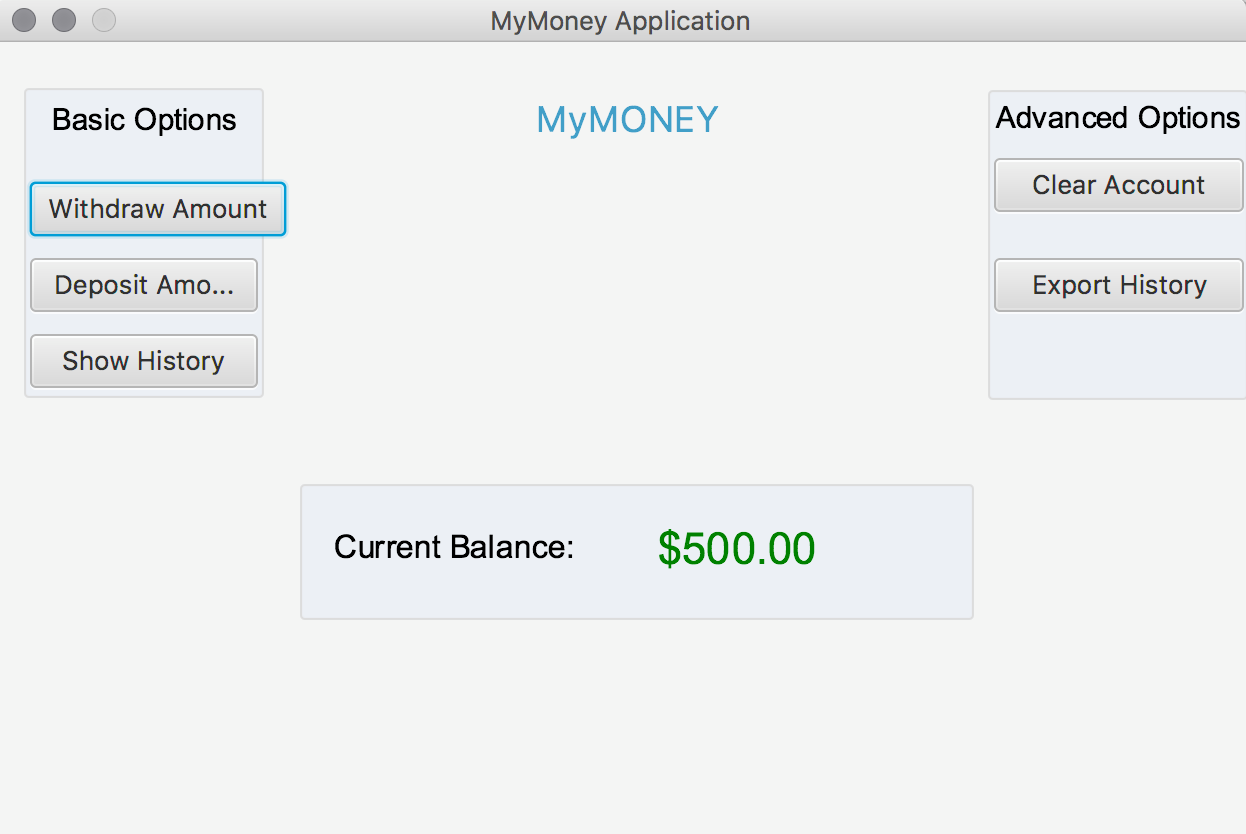
\includegraphics[width=\linewidth]{open_app.png}
  \caption{The user opens myMoney App.}
\end{figure}

\begin{figure}[H]
  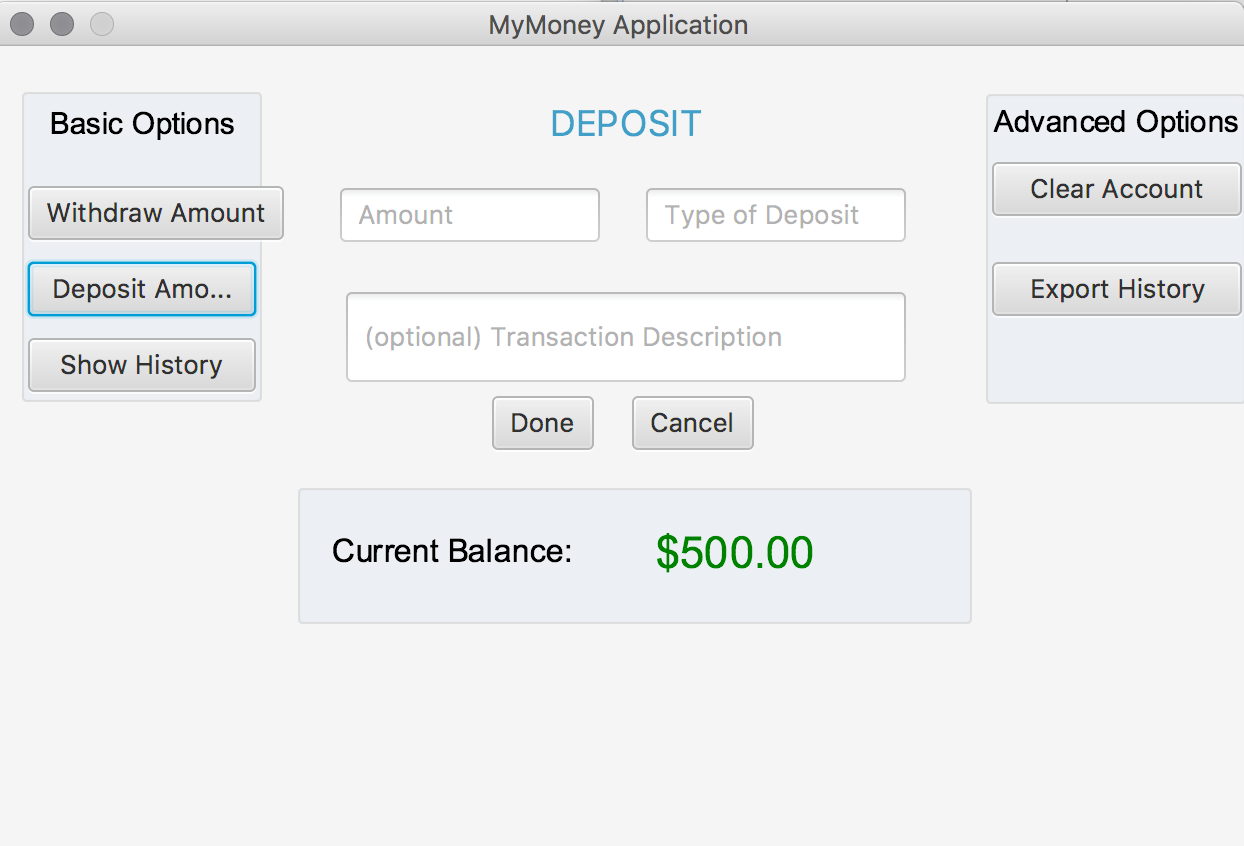
\includegraphics[width=\linewidth]{deposit_click.png}
  \caption{The fields mentioned in the Deposit Test Case section are shown above.}
\end{figure}

\end{document}
